\documentclass{article}
\usepackage[utf8]{inputenc}
\usepackage{graphicx}
\usepackage{amsmath}
\usepackage{hyperref}
\usepackage{listings} 

\setlength{\parindent}{0pt}
\setlength{\parskip}{\baselineskip}

\title{Reversing a charged crossbow's first-person effects on the item model}
\date{February 2022}

\begin{document}

\maketitle

\newpage

\section{Introduction}
When a crossbow is charged, it is centered on the screen in the first-person perspective. The third-person pose also changes, which can be useful when creating custom items via resource packs.

\begin{figure}[h]
	\centering
	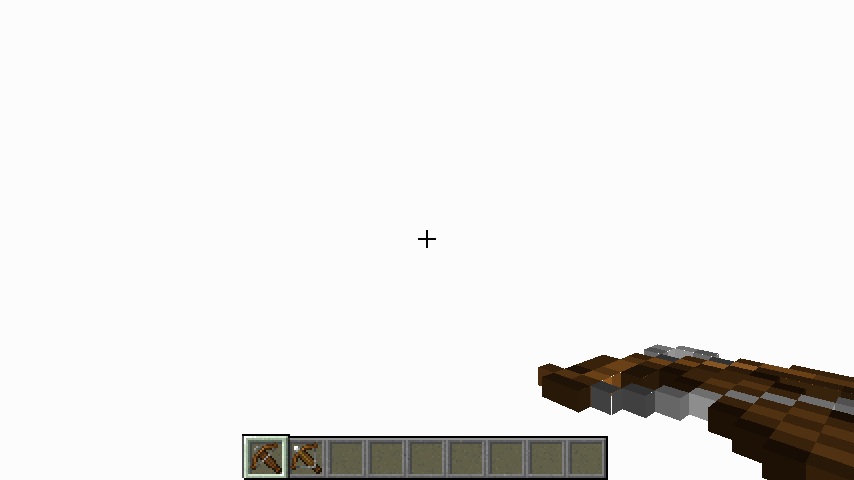
\includegraphics[width=0.75\linewidth]{images/crossbow-stationary}
	\caption{A stationary crossbow.}
	\label{fig:crossbow-stationary}
\end{figure}

\begin{figure}[h]
	\centering
	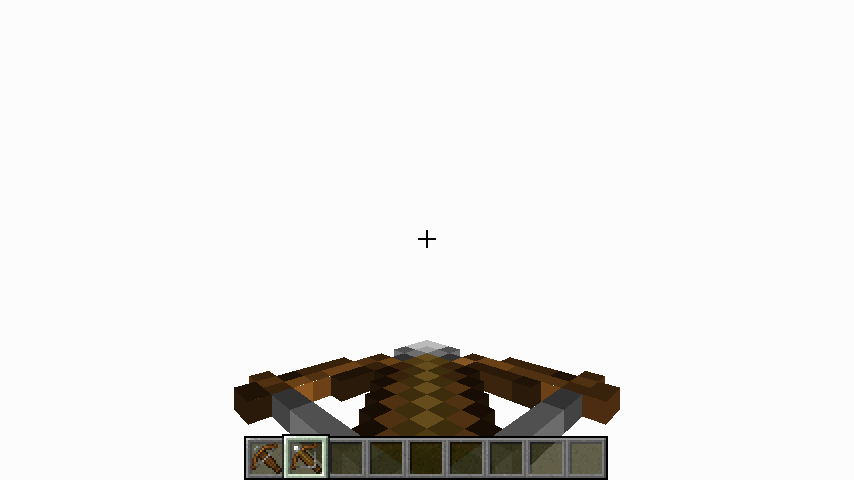
\includegraphics[width=0.75\linewidth]{images/crossbow-charged}
	\caption{A charged crossbow that is centered horizontally on the screen.}
	\label{fig:crossbow-charged}
\end{figure}

\section{What effects are applied?}
\begin{flushleft}\textit{The following numbers were discovered by reading the game code.}\end{flushleft}

The model is moved to the left by a $10.269824$. This is what centres the crossbow on the screen. Furthermore, a $10^{\circ}$ rotation is applied in the y-rotation (yaw).

\section{Reversing the effects}
First, the translation must be reversed. Translations to the left are negative values in x. To reverse this we must add $10.269824$ to the x-translation of the model's display settings for the first-person perspective.

Second, the rotation must be reversed. The y rotation must be subtracted by $10$ to reverse the positive $10^{\circ}$ rotation.

The rotation although means that the translation will now be rotated. To reverse this we must rotate the translation by multiplying it by a rotation matrix. This rotation matrix is the following:

\begin{bmatrix}
$\cos -10^{\circ}$ & 0 & $\sin -10^{\circ}$\\
0 & 1 & 0 \\
$-\sin -10^{\circ}$ & 0 & $\cos -10^{\circ}$
\end{bmatrix}

This is a rotation matrix for rotation around the y-axis (yaw). Source: $R_y(\theta)$ where $\theta=-10^{\circ}$ from \url{https://en.wikipedia.org/wiki/Rotation_matrix#Basic_rotations} [Read 2022-02-01]

To multiply the translation with this matrix, the following can be used to calculate the new x and z translation (y is unchanged).

\begin{cases}
$$\text{newX}=\cos -10^{\circ}\cdot x+\sin -10^{\circ}\cdot z$$ \\
$$\text{newZ}=-\sin -10^{\circ}\cdotx+\cos -10^{\circ}\cdot z$$
\end{cases}

This equates to approximately:

\begin{cases}
$$\text{newX}=0.98480775301\cdot x-0.17364817766\cdot z$$ \\
$$\text{newZ}=0.17364817766\cdot x+0.98480775301\cdot z$$
\end{cases}

\newpage
\section{Example}

\begin{figure}[h]
    \centering
    \begin{lstlisting}
{
  "parent": "example:item/foo",
  "display": {
    "firstperson_righthand": {
      "rotation": [0, 90, 0],
      "translation": [5, 8, 12]
    }
  }
}
    \end{lstlisting}
    \caption{Example model for a normal item}
    \label{fig:example-normal}
\end{figure}

\begin{figure}[h]
    \centering
    \begin{lstlisting}
{
  "parent": "example:item/foo",
  "display": {
    "firstperson_righthand": {
      "rotation": [0, 80, 0],
      "translation": [12.954062930378171, 8, 14.469270146908931]
    }
  }
}
    \end{lstlisting}
    \caption{The same example model, but with the crossbow effects reversed as per the instructions in this paper}
    \label{fig:example-reversed-effects}
\end{figure}

The model in Figure \ref{fig:example-reversed-effects} should be used as a model on a charged crossbow, for example with custom-model-data:
\begin{lstlisting}[escapechar=\%]
"overrides": [
  [...]
  {
    "predicate": {
      "custom_model_data": 100,
      "pulling": 1
    },
    "model": "example:item/Figure_%\ref{fig:example-reversed-effects}%.json"
  }
]
\end{lstlisting}

The model in Figure \ref{fig:example-normal} on any other, normal item should look identical to a charged crossbow with the model from Figure \ref{fig:example-reversed-effects} in the first person right hand perspective. The centering and $10^{\circ}$ rotation has been successfully reversed.

\end{document}
